% Section 5 - MATLAB
% Alessandro Tenaglia <alessandro.tenaglia@uniroma2.it>
% May 6, 2022

% ### MATLAB ###
\section{MATLAB Coder}
\graphicspath{{figs/section5/}}

% --- Model creation ---
\begin{frame}{Model creation}
	\begin{itemize}
		\item Create the model paying attention to data types;
		\item Define inputs as \textbg{Inport blocks} and name them;
		\item Define outputs as \textbg{Outport blocks} and name them;
	\end{itemize}
	\vspace{0.5cm}
	\begin{figure}
		\centering
		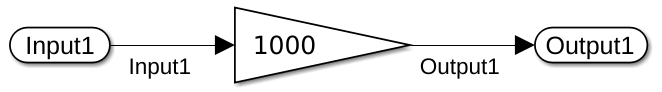
\includegraphics[scale=0.4]{Model.png}
		\label{fig:model}
		\caption{Base model}
	\end{figure}
\end{frame}

% --- Param configuration ---
\begin{frame}{Param configuration}
	Paramters can be:
	\begin{itemize}
		\item \textbg{static}, so no longer modifiable after the code generation;
		\item \textbg{tunable}, so they can be modified at runtime;
	\end{itemize}
	\vspace{0.5cm}
	\begin{figure}
		\centering
		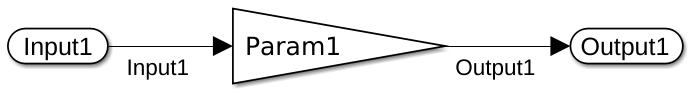
\includegraphics[scale=0.4]{ModelParam.png}
		\label{fig:model_param}
		\caption{Base model with a tunable parameter}
	\end{figure}
\end{frame}

% --- Code generation ---
\begin{frame}{Code generation}
	\begin{figure}
		\centering
		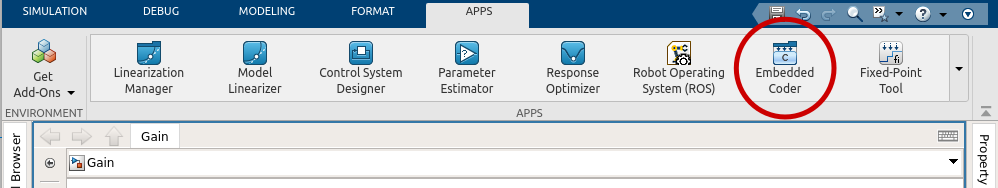
\includegraphics[width=\textwidth]{Embedded.png}
		\label{fig:embedded}
		\caption{Embedded coder app}
	\end{figure}
\end{frame}

% --- Code generation ---
\begin{frame}{Code generation}
	\begin{figure}
		\centering
		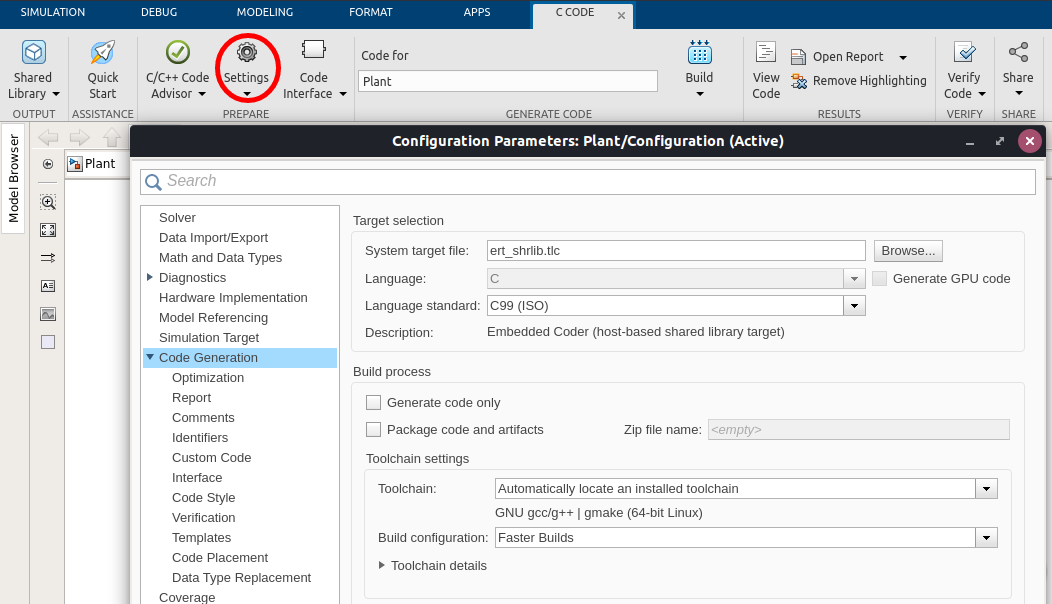
\includegraphics[scale=0.3]{Settings.png}
		\label{fig:settingd}
		\caption{Code generation settings}
	\end{figure}
\end{frame}

% --- Code generation ---
\begin{frame}{Code generation}
	\begin{figure}
		\centering
		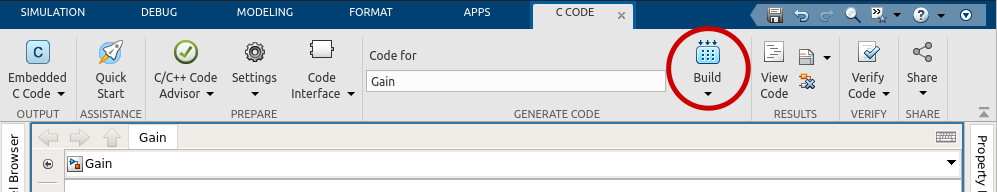
\includegraphics[width=\textwidth]{Build.png}
		\label{fig:build}
		\caption{Base model with tunable parameter}
	\end{figure}
\end{frame}

% --- SimulinkWrapperGAM ---
\begin{frame}[fragile]{Configuration file: SimulinkWrapperGAM}
	\begin{columns}\column{.8\textwidth}
		\begin{lstlisting}[style=small, language = cfg]
+GAMGain = {
    Class = SimulinkWrapperGAM
    Library = Gain.so // Library name
    SymbolPrefix = Gain // Model name
    InputSignals = {
        Input1 = {
            DataSource = DDB1
            Type = int32
        }
    }
    OutputSignals = {
        Output1 = {
            DataSource = DDB1
            Type = int32
        }
    }
    Parameters = {
        Param1 = (int32) 1000
    }
}\end{lstlisting}
	\end{columns}
\end{frame}

% --- Example: Control System ---
\begin{frame}{Example: Control System}
	\begin{figure}
		\centering
		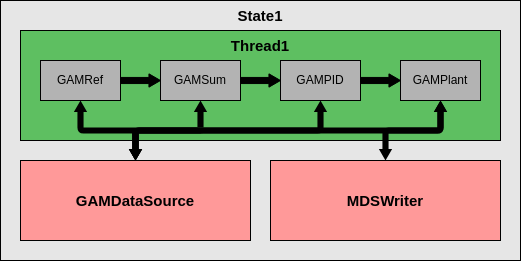
\includegraphics[scale=0.55]{ControlSystem.png}
		\label{fig:control}
		\caption{Control system app scheme}
	\end{figure}
\end{frame}
